% This file was created with tikzplotlib v0.9.12.
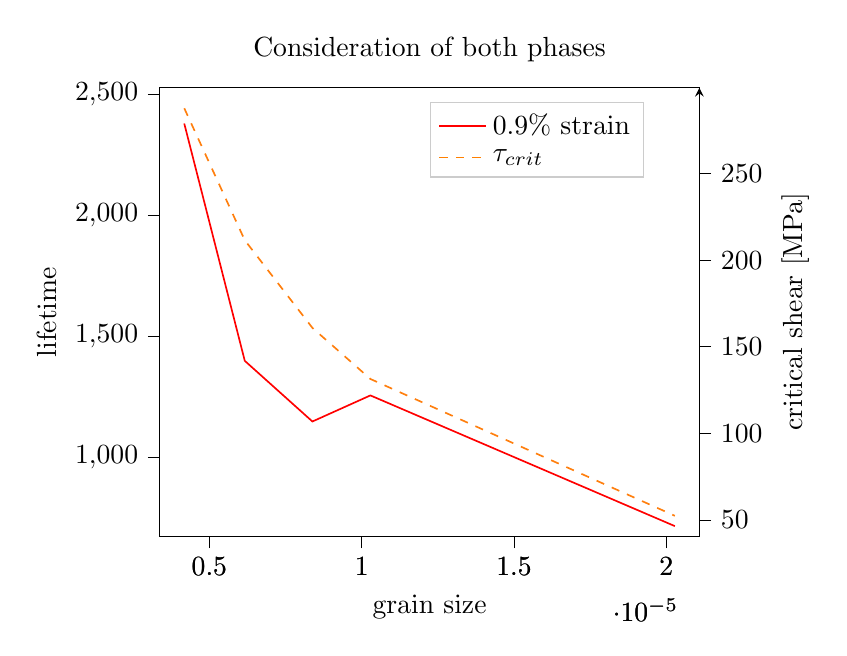
\begin{tikzpicture}[baseline]

\definecolor{color0}{rgb}{1,0.498039215686275,0.0549019607843137}

\begin{axis}[
legend cell align={left},
legend style={
  fill opacity=0.8,
  draw opacity=1,
  text opacity=1,
  at={(0.5,0.8)},
  anchor=south west,
  draw=white!80!black
},
log basis y={10},
tick align=outside,
tick pos=left,
x grid style={white!69.0196078431373!black},
xlabel={grain size},
xmin=3.36954929815941e-06, xmax=2.10882960351094e-05,
xtick style={color=black},
y grid style={white!69.0196078431373!black},
ylabel={lifetime},
ymin=671.697168907907, ymax=2525.38343877006,
scaled y ticks = true,
%ymode=log,
ytick style={color=black}
]
\addplot [semithick, red]
table {%
4.17494687711168e-06 2377.84736188214
6.16182238274221e-06 1396.75098868979
8.38251085785529e-06 1145.92034700236
1.02863466506117e-05 1253.76197072447
2.02828984561571e-05 713.373336497974
};
\addlegendentry{0.9\% strain}
\addlegendimage{dashed,orange}
\addlegendentry{$\tau_{crit}$}
\end{axis}

\begin{axis}[
axis y line=right,
tick align=outside,
title={Consideration of both phases},
x grid style={white!69.0196078431373!black},
xmin=3.36954929815941e-06, xmax=2.10882960351094e-05,
xtick pos=left,
xtick style={color=black},
y grid style={white!69.0196078431373!black},
ylabel={critical shear [MPa]},
ymin=40.635, ymax=299.465,
ytick pos=right,
ytick style={color=black},
yticklabel style={anchor=west}
]
\addplot [semithick, color0, dashed]
table {%
4.17494687711168e-06 287.7
6.16182238274221e-06 211.5
8.38251085785529e-06 160.9
1.02863466506117e-05 131.4
2.02828984561571e-05 52.4
};
%\addlegendentry{$\tau_{crit}$}
\end{axis}

\end{tikzpicture}
